\renewcommand{\tema}{Lección: Óptica}

% ============================================================
%  SECCIÓN 1: LA LUZ Y SUS MODELOS
% ============================================================

\section{La Luz y sus Modelos}

\begin{seccion}
La naturaleza de la luz ha sido una de las preguntas más persistentes de la física. Durante siglos, dos modelos rivales explicaron sus comportamientos de formas incompatibles entre sí. La resolución de esa tensión llevó, en el siglo XX, a uno de los conceptos más profundos de la física moderna: el fotón.
\end{seccion}

\subsection{Modelo corpuscular de Newton}

\begin{seccion}
\begin{definicion}
\textbf{Modelo corpuscular (Newton, siglo XVII):} La luz está formada por pequeñas partículas llamadas \textit{corpúsculos} que viajan en línea recta a gran velocidad. Cada color corresponde a corpúsculos de diferente tamaño o velocidad.
\end{definicion}

Este modelo explica con elegancia la propagación rectilínea de la luz y la formación de sombras nítidas. También predice la reflexión de forma natural: los corpúsculos rebotan en las superficies como pelotas elásticas.

\textbf{Éxitos del modelo:}
\begin{itemize}
    \item Propagación en línea recta.
    \item Reflexión (rebote de partículas).
    \item Separación de colores al pasar por un prisma.
\end{itemize}

\textbf{Limitación principal:} Predice que la luz debería viajar \textit{más rápido} en medios densos como el agua, lo cual resultó ser falso al medirse experimentalmente.
\end{seccion}

\subsection{Modelo ondulatorio de Huygens}

\begin{seccion}
\begin{definicion}
\textbf{Modelo ondulatorio (Huygens, siglo XVII):} La luz es una onda que se propaga en el espacio. Cada punto de un frente de onda actúa como fuente de ondas secundarias esféricas; la envolvente de estas ondas secundarias forma el nuevo frente de onda.
\end{definicion}

Este modelo, conocido como \textbf{principio de Huygens}, explica fenómenos que el modelo corpuscular no puede: la difracción (la luz se dobla alrededor de obstáculos), la interferencia (dos haces de luz pueden cancelarse) y la refracción correcta (la luz va \textit{más lento} en medios densos).

\textbf{Éxitos del modelo:}
\begin{itemize}
    \item Difracción e interferencia.
    \item Refracción con la velocidad correcta en cada medio.
    \item Explica la doble refracción en cristales.
\end{itemize}
\end{seccion}

\subsubsection{Diagrama: Principio de Huygens}

\begin{center}
\begin{tikzpicture}[scale=1.0]

\draw[azuloscuro, very thick] (0, -2.5) -- (0, 2.5);
\node[left, font=\footnotesize, color=azuloscuro] at (-0.1, 2.7) {frente de onda};

\foreach \y in {-2.0, -1.0, 0.0, 1.0, 2.0} {
    \fill[azuloscuro] (0, \y) circle (0.07);
    \draw[azulmedio!60, thin] (0, \y) circle (0.6);
    \draw[azulmedio!40, thin] (0, \y) circle (1.1);
}

\draw[verdecorrecto, very thick] (1.1, -2.5) -- (1.1, 2.5);
\node[right, font=\footnotesize, color=verdecorrecto] at (1.2, 2.7) {nuevo frente};

\foreach \y in {-1.5, 0.0, 1.5} {
    \draw[-{Stealth}, azuloscuro, thick] (1.15, \y) -- (2.0, \y);
}
\node[right, font=\footnotesize, color=azuloscuro] at (2.05, 0) {propagación};

\draw[->, thin, gray] (0.7, -2.3) -- (0.05, -2.0);
\node[right, font=\footnotesize, color=gray] at (0.75, -2.3) {fuentes secundarias};

\end{tikzpicture}
\end{center}

\subsection{El fotón: síntesis moderna}

\begin{seccion}
\begin{definicion}
\textbf{Fotón (Einstein, 1905):} La luz está formada por cuantos de energía llamados \textit{fotones}. Cada fotón transporta una energía proporcional a la frecuencia de la radiación:
$$E = h \cdot f$$
donde $h = 6.626 \times 10^{-34}$ J$\cdot$s es la constante de Planck y $f$ es la frecuencia.
\end{definicion}

La física moderna acepta que la luz tiene \textbf{dualidad onda-partícula}: se comporta como onda en fenómenos de interferencia y difracción, y como partícula (fotón) en la interacción con la materia (efecto fotoeléctrico, visión, fotografía).

\begin{nota}
\textbf{Es importante recordar que} para el examen de admisión solo se requiere saber que la luz es una onda electromagnética transversal, que viaja a $c = 3 \times 10^8$ m/s en el vacío, y que diferentes colores corresponden a diferentes frecuencias (y longitudes de onda). La ecuación del fotón $E = hf$ aparece ocasionalmente en preguntas conceptuales.
\end{nota}
\end{seccion}

\subsubsection{Diagrama: Espectro electromagnético visible}

\begin{center}
\begin{tikzpicture}[scale=1.0]

\fill[violet!80]       (0.0, 0) rectangle (1.2, 0.7);
\fill[blue!70]         (1.2, 0) rectangle (2.4, 0.7);
\fill[cyan!60!blue]    (2.4, 0) rectangle (3.6, 0.7);
\fill[green!60]        (3.6, 0) rectangle (4.8, 0.7);
\fill[yellow!80]       (4.8, 0) rectangle (6.0, 0.7);
\fill[orange!80]       (6.0, 0) rectangle (7.2, 0.7);
\fill[red!80]          (7.2, 0) rectangle (8.4, 0.7);

\draw[thick, gray] (0,0) rectangle (8.4, 0.7);

\node[font=\tiny, white] at (0.6,  0.35) {violeta};
\node[font=\tiny, white] at (1.8,  0.35) {azul};
\node[font=\tiny, black] at (3.0,  0.35) {cian};
\node[font=\tiny, black] at (4.2,  0.35) {verde};
\node[font=\tiny, black] at (5.4,  0.35) {amarillo};
\node[font=\tiny, black] at (6.6,  0.35) {naranja};
\node[font=\tiny, white] at (7.8,  0.35) {rojo};

\draw[-{Stealth}, thick] (0, -0.2) -- (8.6, -0.2)
    node[right, font=\small] {$\lambda$ (nm)};
\foreach \x/\lam in {0/380, 1.2/430, 2.4/470, 3.6/500, 4.8/560, 6.0/590, 7.2/620, 8.4/700} {
    \draw[thin] (\x, -0.15) -- (\x, -0.25);
    \node[below, font=\tiny] at (\x, -0.25) {\lam};
}

\draw[-{Stealth}, thick] (8.4, -0.85) -- (0, -0.85)
    node[left, font=\small] {$f$ (Hz)};
\node[font=\footnotesize, color=gray] at (4.2, -1.2)
    {mayor $\lambda$ $\Leftrightarrow$ menor $f$ $\Leftrightarrow$ menor energía};

\end{tikzpicture}
\end{center}

% ============================================================
%  SECCIÓN 2: REFLEXIÓN DE LA LUZ
% ============================================================

\section{Reflexión de la Luz}

\begin{seccion}
La reflexión es el fenómeno por el cual la luz rebota al incidir sobre una superficie. Es el principio que permite ver los objetos que no emiten luz propia: vemos una silla porque la luz del sol o de una lámpara rebota en ella y llega a nuestros ojos.
\end{seccion}

\subsection{Reflexión en superficie lisa y rugosa}

\begin{seccion}
\begin{definicion}
\textbf{Reflexión especular:} Ocurre en superficies lisas (espejo, agua tranquila). Los rayos incidentes paralelos se reflejan de forma paralela, produciendo una imagen nítida.
\end{definicion}

\begin{definicion}
\textbf{Reflexión difusa:} Ocurre en superficies rugosas (papel, pared, madera). Los rayos incidentes paralelos se reflejan en múltiples direcciones. No se forma imagen, pero la superficie es visible desde cualquier ángulo.
\end{definicion}

Es importante recordar que ambos tipos de reflexión obedecen la misma ley de reflexión en cada punto de la superficie. La diferencia es que en la superficie rugosa, la normal varía en cada punto, por lo que los rayos reflejados salen en direcciones distintas.
\end{seccion}

\subsubsection{Diagrama: Reflexión especular y difusa}

\begin{center}
\begin{tikzpicture}[scale=1.0]

\node[font=\bfseries\small, color=azuloscuro] at (1.5, 3.2) {Reflexión especular};

\draw[very thick, azuloscuro] (0, 0) -- (3, 0);
\foreach \x in {0.1, 0.5, ..., 2.9} {
    \draw[gray!40, thin] (\x, 0) -- (\x-0.2, -0.2);
}

\foreach \xo/\xi in {0.3/0.8, 0.9/1.4, 1.5/2.0} {
    \draw[-{Stealth}, azulmedio, thick] (\xo, 2.5) -- (\xi, 0);
}

\foreach \xi/\xr in {0.8/1.3, 1.4/1.9, 2.0/2.5} {
    \draw[-{Stealth}, verdecorrecto, thick] (\xi, 0) -- (\xr, 2.5);
}

\node[font=\bfseries\small, color=azuloscuro] at (6.5, 3.2) {Reflexión difusa};

\draw[very thick, azuloscuro]
    (4.0,0) -- (4.4,0.15) -- (4.8,-0.1) -- (5.2,0.2) --
    (5.6,-0.05) -- (6.0,0.18) -- (6.4,-0.12) -- (6.8,0.1) -- (7.2,0.0) -- (7.5,0);
\foreach \x in {4.1, 4.5, ..., 7.4} {
    \draw[gray!40, thin] (\x, -0.05) -- (\x-0.2, -0.25);
}

\foreach \xo/\xi/\yi in {4.5/5.0/0.12, 5.3/5.7/-0.03, 6.2/6.5/0.14} {
    \draw[-{Stealth}, azulmedio, thick] (\xo, 2.5) -- (\xi, \yi);
}

\draw[-{Stealth}, verdecorrecto, thick] (5.0,0.12) -- (4.4, 2.2);
\draw[-{Stealth}, verdecorrecto, thick] (5.0,0.12) -- (5.5, 2.4);
\draw[-{Stealth}, verdecorrecto, thick] (5.7,-0.03) -- (5.0, 2.3);
\draw[-{Stealth}, verdecorrecto, thick] (5.7,-0.03) -- (6.4, 2.1);
\draw[-{Stealth}, verdecorrecto, thick] (6.5,0.14) -- (6.0, 2.4);
\draw[-{Stealth}, verdecorrecto, thick] (6.5,0.14) -- (7.1, 2.2);

\end{tikzpicture}
\end{center}

\subsection{Ley de reflexión}

\begin{seccion}
\begin{definicion}
\textbf{Ley de reflexión:} El rayo incidente, la normal a la superficie en el punto de incidencia y el rayo reflejado son coplanares. El ángulo de incidencia es igual al ángulo de reflexión, ambos medidos respecto a la normal.
\end{definicion}

\begin{ecuacion}
$$\theta_i = \theta_r$$

donde:
\begin{itemize}
    \item $\theta_i$ = ángulo de incidencia (entre el rayo incidente y la normal)
    \item $\theta_r$ = ángulo de reflexión (entre el rayo reflejado y la normal)
\end{itemize}
\end{ecuacion}

\textbf{Consecuencias importantes:}
\begin{itemize}
    \item Si el rayo incide perpendicularmente a la superficie ($\theta_i = 0$), se refleja de regreso por el mismo camino.
    \item El ángulo se mide siempre respecto a la \textbf{normal}, no respecto a la superficie.
    \item La ley aplica tanto para reflexión especular como para cada punto de una superficie difusa.
\end{itemize}
\end{seccion}

\subsubsection{Diagrama: Ley de reflexión}

\begin{center}
\begin{tikzpicture}[scale=1.2]

\draw[very thick, azuloscuro] (-3.2, 0) -- (3.2, 0);
\foreach \x in {-3.0,-2.5,...,3.0} {
    \draw[gray!40, thin] (\x, 0) -- (\x-0.3, -0.3);
}

\draw[dashed, gray, thick] (0, -1.0) -- (0, 2.5);
\node[right, font=\footnotesize, color=gray] at (0.05, 2.3) {normal};

\draw[-{Stealth}, very thick, azulmedio] (-2.5, 2.2) -- (0, 0);
\node[left, font=\small, color=azulmedio] at (-1.8, 1.6) {rayo incidente};

\draw[-{Stealth}, very thick, verdecorrecto] (0, 0) -- (2.5, 2.2);
\node[right, font=\small, color=verdecorrecto] at (1.8, 1.6) {rayo reflejado};

\draw[azulmedio, thin] (0, 0.8) arc (90:138.8:0.8);
\node[font=\small, color=azulmedio] at (-0.6, 1.05) {$\theta_i$};

\draw[verdecorrecto, thin] (0, 0.8) arc (90:41.2:0.8);
\node[font=\small, color=verdecorrecto] at (0.6, 1.05) {$\theta_r$};

\node[font=\normalsize, color=azuloscuro] at (0, -0.7) {$\theta_i = \theta_r$};

\end{tikzpicture}
\end{center}

% ============================================================
%  SECCIÓN 3: REFRACCIÓN DE LA LUZ — LEY DE SNELL
% ============================================================

\section{Refracción de la Luz}

\begin{seccion}
Cuando la luz pasa de un medio a otro con diferente velocidad de propagación, cambia de dirección. Este fenómeno se llama refracción y es responsable de una enorme variedad de efectos cotidianos: desde la cuchara que parece rota en un vaso de agua hasta la formación de arcoíris, el funcionamiento de los lentes de los anteojos y el diseño de las fibras ópticas.
\end{seccion}

\subsection{Índice de refracción}

\begin{seccion}
\begin{definicion}
\textbf{Índice de refracción} ($n$): cociente entre la velocidad de la luz en el vacío ($c$) y la velocidad de la luz en el medio ($v$).
\end{definicion}

\begin{ecuacion}
$$n = \frac{c}{v}$$

donde:
\begin{itemize}
    \item $c = 3 \times 10^8$ m/s (velocidad de la luz en el vacío)
    \item $v$ = velocidad de la luz en el medio
    \item $n \geq 1$ siempre (la luz nunca va más rápido que en el vacío)
\end{itemize}
\end{ecuacion}

\textbf{Valores de referencia:}

\begin{center}
\begin{tabular}{lc}
\hline
\rowcolor{fondogris}
\textbf{Medio}   & \textbf{Índice de refracción $n$} \\
\hline
Vacío            & 1.000 \\
Aire             & 1.0003 $\approx$ 1 \\
Agua             & 1.33 \\
Vidrio crown     & 1.52 \\
Diamante         & 2.42 \\
\hline
\end{tabular}
\end{center}

\begin{nota}
\textbf{Nota:} Un índice de refracción mayor significa que la luz viaja más \textit{lento} en ese medio. El diamante tiene el índice más alto de los materiales comunes, lo que produce su característica destellante al doblar la luz con gran ángulo.
\end{nota}
\end{seccion}

\subsection{Ley de Snell}

\begin{seccion}
\begin{definicion}
\textbf{Ley de Snell (o ley de Snell-Descartes):} Al pasar de un medio con índice $n_1$ a uno con índice $n_2$, los ángulos de incidencia y refracción satisfacen:
\end{definicion}

\begin{ecuacion}
$$n_1 \cdot \sin\theta_1 = n_2 \cdot \sin\theta_2$$

donde $\theta_1$ y $\theta_2$ se miden respecto a la normal en la superficie de separación.
\end{ecuacion}

\textbf{Reglas que se deducen directamente de la ley de Snell:}
\begin{itemize}
    \item Si $n_2 > n_1$ (pasa a medio más denso): $\theta_2 < \theta_1$ — el rayo \textbf{se acerca} a la normal.
    \item Si $n_2 < n_1$ (pasa a medio menos denso): $\theta_2 > \theta_1$ — el rayo \textbf{se aleja} de la normal.
    \item La frecuencia de la luz \textbf{no cambia} al refractarse; solo cambian $v$ y $\lambda$.
\end{itemize}
\end{seccion}

\subsubsection{Diagrama: Ley de Snell}

\begin{center}
\begin{tikzpicture}[scale=1.15]

\fill[azulmedio!8] (-3.5, 0) rectangle (3.5, 3.0);
\node[font=\small, color=azuloscuro] at (-2.8, 0.6) {Medio 1};
\node[font=\footnotesize, color=azuloscuro] at (-2.1, 0.2) {(velocidad $v_1$, mayor)};

\fill[azulmedio!22] (-3.5, -2.8) rectangle (3.5, 0);
\node[font=\small, color=azuloscuro] at (-2.8, -0.3) {Medio 2};
\node[font=\footnotesize, color=azuloscuro] at (-2.1, -0.7) {(velocidad $v_2$, menor)};

\draw[very thick, color=azuloscuro] (-3.5, 0) -- (3.5, 0);
\foreach \x in {-3.3,-2.9,...,3.3} {
    \draw[gray!40, thin] (\x, 0) -- (\x+0.3, -0.3);
}

\draw[dashed, gray, thick] (0, -2.6) -- (0, 2.8);
\node[right, font=\footnotesize, color=gray] at (0.05, 2.5) {normal};

\draw[-{Stealth}, very thick, color=azulmedio] (-2.4, 2.6) -- (0, 0);
\node[left, font=\small, color=azulmedio] at (-1.7, 1.8) {rayo incidente};

\draw[-{Stealth}, thick, color=azulmedio!50, dashed] (0, 0) -- (2.4, 2.6);
\node[right, font=\footnotesize, color=azulmedio!70] at (1.8, 1.8) {reflejado};

\draw[-{Stealth}, very thick, color=verdecorrecto] (0, 0) -- (1.4, -2.6);
\node[right, font=\small, color=verdecorrecto] at (1.0, -1.6) {rayo refractado};

\draw[color=azulmedio, thin] (0, 0.8) arc (90:132:0.8);
\node[font=\footnotesize, color=azulmedio] at (-0.55, 1.0) {$\theta_1$};

\draw[color=verdecorrecto, thin] (0,-0.8) arc (270:297:0.8);
\node[font=\footnotesize, color=verdecorrecto] at (0.3, -1.05) {$\theta_2$};

\node[font=\footnotesize, color=gray!80] at (2.5, -0.5) {$\theta_2 < \theta_1$};
\node[font=\footnotesize, color=gray!80] at (2.5, -0.9) {(medio más lento)};

\end{tikzpicture}
\end{center}

\subsection{Efectos cotidianos de la refracción}

\begin{seccion}
\begin{itemize}
    \item \textbf{Cuchara rota:} Una cuchara sumergida en agua parece doblada en la superficie. La luz que viene de la parte sumergida cambia de dirección al pasar del agua al aire, desplazando aparentemente la imagen.
    \item \textbf{Arcoíris:} Las gotas de lluvia refractan la luz dos veces (al entrar y al salir) y la reflejan internamente. Dado que el índice de refracción del agua depende de la frecuencia (longitud de onda), cada color se desvía un ángulo distinto, separando la luz blanca en el espectro.
    \item \textbf{Espejismo:} En carreteras muy calientes, el aire cerca del asfalto está más caliente y tiene menor índice de refracción que el aire frío superior. La luz se curva hacia arriba, produciendo la ilusión de un charco de agua.
    \item \textbf{Fibra óptica:} La luz viaja confinada dentro de un hilo de vidrio porque al incidir con ángulo rasante sobre la pared, el ángulo es mayor que el ángulo crítico y se produce reflexión total interna — la luz no puede escapar.
    \item \textbf{Lentes de anteojos:} Las lentes curvan los rayos de luz por refracción para compensar defectos de visión. Una lente convergente acerca los rayos hacia el eje; una divergente los separa.
\end{itemize}
\end{seccion}

\subsection{Ejercicios resueltos: ley de Snell e índice de refracción}

\begin{seccion}

\textbf{Ejercicio 1.} Un rayo de luz pasa del aire ($n_1 = 1$) al vidrio ($n_2 = 1.5$) con un ángulo de incidencia de $30^\circ$. ¿Cuál es el ángulo de refracción?

\begin{ecuacion}
\textbf{Fórmula:} $n_1 \sin\theta_1 = n_2 \sin\theta_2$

\textbf{Sustitución:}
$$1 \cdot \sin 30^\circ = 1.5 \cdot \sin\theta_2$$
$$0.5 = 1.5 \cdot \sin\theta_2$$
$$\sin\theta_2 = \frac{0.5}{1.5} = \frac{1}{3} \approx 0.333$$
$$\theta_2 = \arcsin(0.333) \approx 19.5^\circ$$

El rayo se acerca a la normal ($\theta_2 < \theta_1$) al pasar a un medio más denso.
\end{ecuacion}

\vspace{0.4cm}

\textbf{Ejercicio 2.} La velocidad de la luz en cierto plástico es $2 \times 10^8$ m/s. ¿Cuál es su índice de refracción?

\begin{ecuacion}
\textbf{Fórmula:} $n = \dfrac{c}{v}$

\textbf{Sustitución:}
$$n = \frac{3 \times 10^8 \text{ m/s}}{2 \times 10^8 \text{ m/s}} = 1.5$$
\end{ecuacion}

\vspace{0.4cm}

\textbf{Ejercicio 3.} Un rayo pasa del agua ($n_1 = 1.33$) al aire ($n_2 = 1$). Si el ángulo de incidencia es $20^\circ$, ¿hacia dónde se desvía el rayo refractado?

\begin{ecuacion}
Como $n_2 < n_1$, la luz pasa a un medio menos denso: el rayo refractado \textbf{se aleja de la normal} ($\theta_2 > \theta_1$).

Verificación:
$$\sin\theta_2 = \frac{n_1}{n_2}\sin\theta_1 = \frac{1.33}{1} \times \sin 20^\circ = 1.33 \times 0.342 = 0.455$$
$$\theta_2 \approx 27^\circ > 20^\circ \quad \checkmark$$
\end{ecuacion}

\begin{nota}
\textbf{Nota:} En el examen de admisión raramente piden calcular $\arcsin$. Lo más común es pedir si el rayo se acerca o se aleja de la normal, o calcular $n$ a partir de velocidades. Memoriza: medio más denso ($n$ mayor) $\Rightarrow$ rayo más cercano a la normal.
\end{nota}

\end{seccion}

% ============================================================
%  SECCIÓN 4: ESPEJOS PLANOS Y ESFÉRICOS
% ============================================================

\section{Espejos Planos y Esféricos}

\begin{seccion}
Los espejos son superficies pulidas que reflejan la luz de forma especular. Según su geometría, forman imágenes con características muy distintas. Los espejos planos producen imágenes del mismo tamaño que el objeto; los espejos curvos pueden ampliar, reducir, invertir o hacer que la imagen sea virtual, dependiendo de dónde se coloque el objeto.
\end{seccion}

\subsection{Espejos planos}

\begin{seccion}
\begin{definicion}
\textbf{Espejo plano:} Superficie reflectante plana. La imagen formada es \textit{virtual} (no se puede proyectar en una pantalla), \textit{derecha} (no invertida verticalmente), del \textit{mismo tamaño} que el objeto, y se forma a la misma distancia detrás del espejo que la distancia del objeto frente a él.
\end{definicion}

\textbf{Propiedades de la imagen en espejo plano:}
\begin{itemize}
    \item Virtual y derecha.
    \item Mismo tamaño que el objeto ($m = 1$).
    \item Distancia imagen = distancia objeto ($d_i = d_o$).
    \item Lateralmente invertida (la mano derecha aparece como izquierda).
\end{itemize}
\end{seccion}

\subsection{Espejos esféricos: elementos}

\begin{seccion}
Un espejo esférico es una sección de una esfera hueca cuya superficie interior (cóncava) o exterior (convexa) está pulida.

\begin{definicion}
\textbf{Espejo cóncavo:} La superficie reflectante es el interior de la esfera. Converge los rayos paralelos en un punto. Se usa en telescopios, faros de automóviles y espejos de maquillaje.
\end{definicion}

\begin{definicion}
\textbf{Espejo convexo:} La superficie reflectante es el exterior de la esfera. Diverge los rayos reflejados. Se usa en espejos de seguridad y retrovisores.
\end{definicion}

\textbf{Elementos de un espejo esférico:}
\begin{itemize}
    \item \textbf{Centro de curvatura} ($C$): centro de la esfera de la que es parte el espejo. Distancia al espejo: $R$.
    \item \textbf{Foco} ($F$): punto donde convergen los rayos paralelos al eje (espejo cóncavo) o desde donde parecen provenir (espejo convexo). Distancia focal: $f = R/2$.
    \item \textbf{Vértice} ($V$): punto central del espejo.
    \item \textbf{Eje principal}: línea que pasa por $C$, $F$ y $V$.
\end{itemize}
\end{seccion}

\subsubsection{Diagrama: Elementos de un espejo esférico}
\begin{center}
    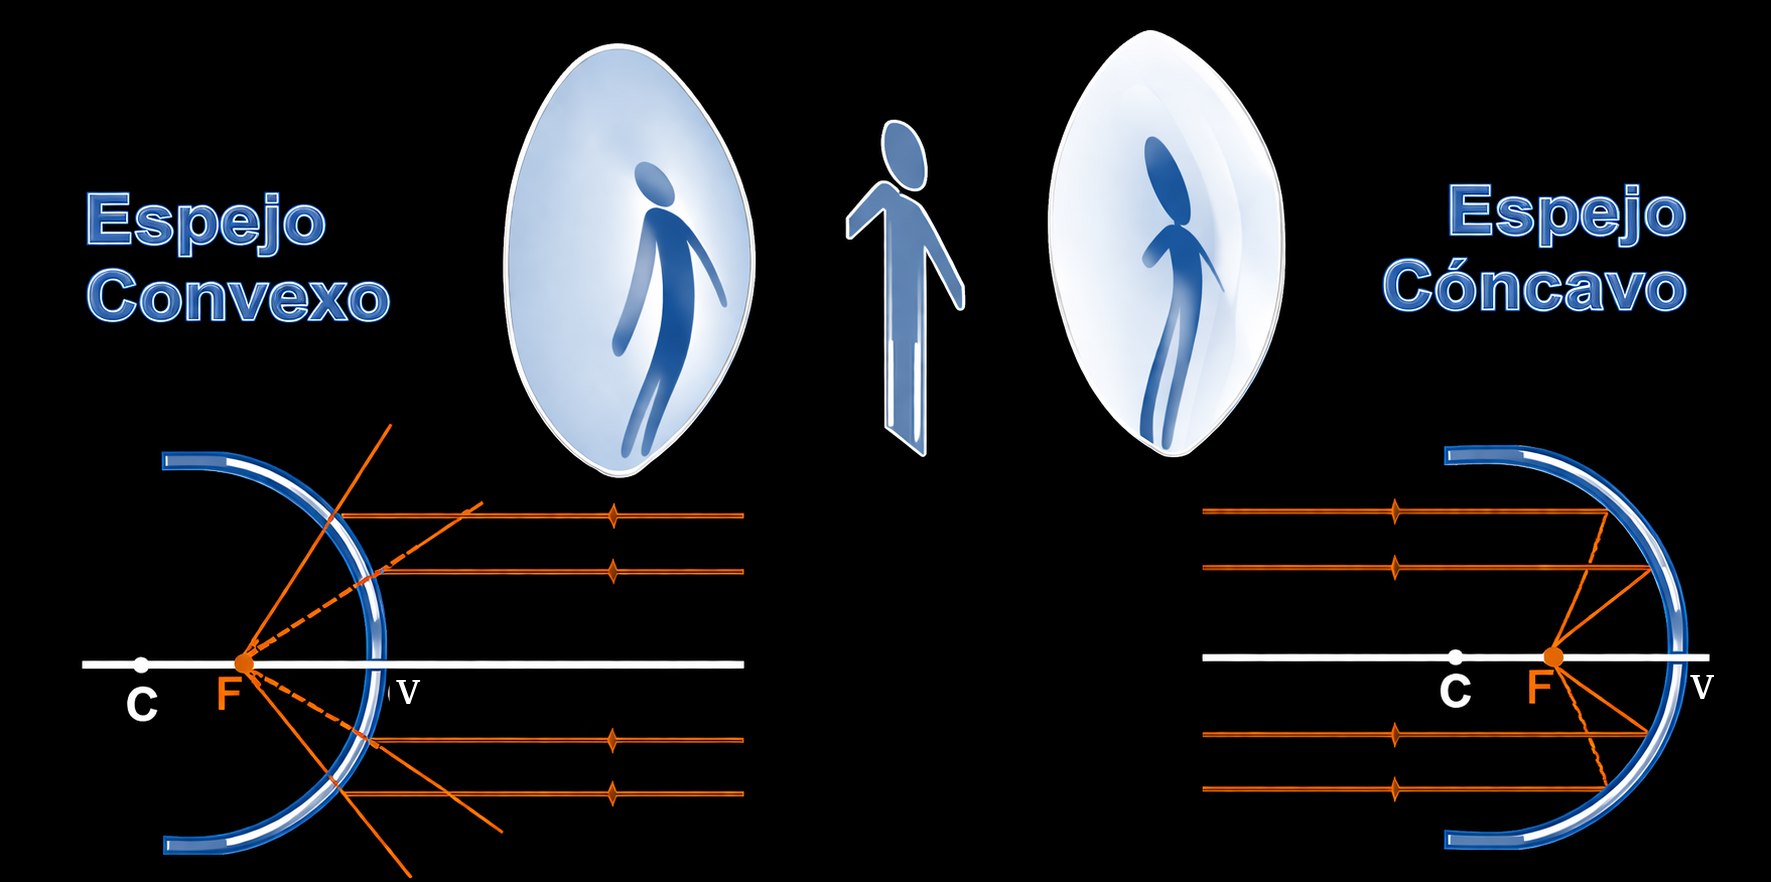
\includegraphics[width=0.70\textwidth]{CLASES/IMAGENES/espejos_esfericos.png}
\end{center}

\subsection{Ecuaciones del espejo esférico}

\begin{seccion}
\begin{ecuacion}
\textbf{Ecuación del espejo:}
$$\frac{1}{f} = \frac{1}{d_o} + \frac{1}{d_i}$$

donde:
\begin{itemize}
    \item $f$ = distancia focal (positiva en cóncavo, negativa en convexo)
    \item $d_o$ = distancia del objeto al espejo (siempre positiva)
    \item $d_i$ = distancia de la imagen al espejo (positiva si es real, negativa si es virtual)
\end{itemize}
\end{ecuacion}

\begin{ecuacion}
\textbf{Aumento lateral} ($m$):
$$m = -\frac{d_i}{d_o}$$

\begin{itemize}
    \item $|m| > 1$: imagen más grande que el objeto.
    \item $|m| < 1$: imagen más pequeña que el objeto.
    \item $m > 0$: imagen derecha (virtual).
    \item $m < 0$: imagen invertida (real).
\end{itemize}
\end{ecuacion}

\textbf{Convención de signos:}
\begin{itemize}
    \item Espejo \textbf{cóncavo}: $f > 0$
    \item Espejo \textbf{convexo}: $f < 0$
    \item Imagen \textbf{real} (frente al espejo): $d_i > 0$
    \item Imagen \textbf{virtual} (detrás del espejo): $d_i < 0$
\end{itemize}
\end{seccion}

\subsubsection{Diagrama: Rayos notables en un espejo cóncavo}

\begin{center}
    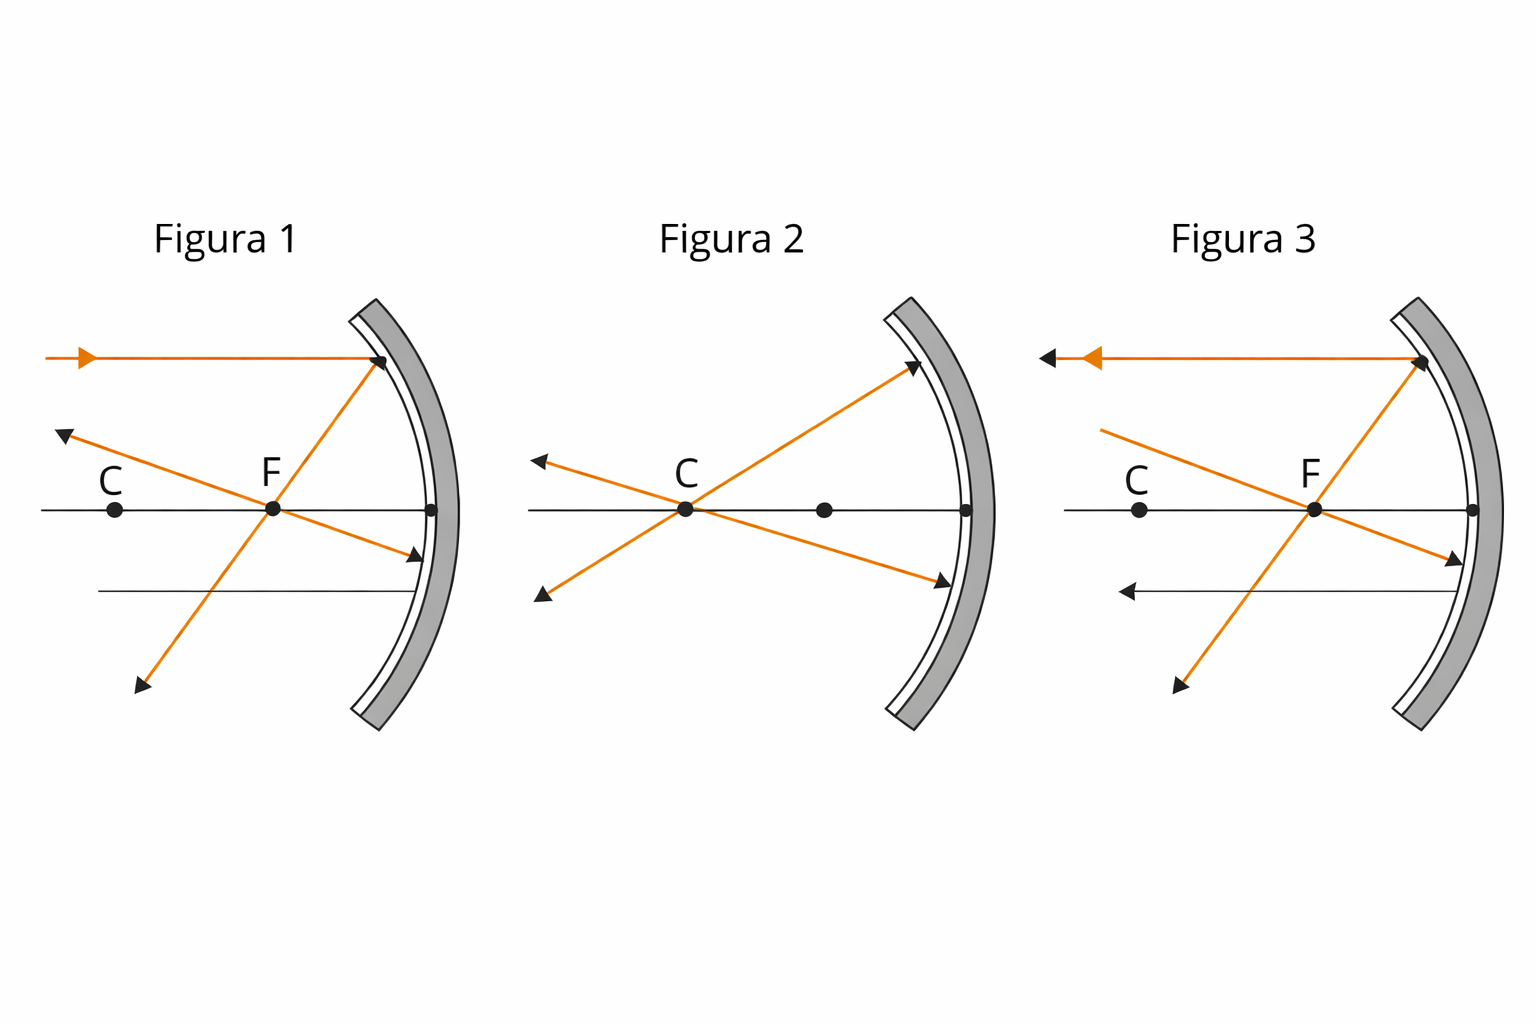
\includegraphics[width=0.70\textwidth]{CLASES/IMAGENES/espejos_concavos.png}
\end{center}

\subsubsection{Diagrama: Formación de imagenes en espejos cóncavos}

\subsection{Ejercicios resueltos: espejos esféricos}

\begin{seccion}

\textbf{Ejercicio 1.} Un objeto se coloca a 30 cm frente a un espejo cóncavo de distancia focal 10 cm. ¿A qué distancia se forma la imagen? ¿Es real o virtual?

\begin{ecuacion}
\textbf{Datos:} $d_o = 30$ cm, $f = 10$ cm

\textbf{Fórmula:} $\dfrac{1}{f} = \dfrac{1}{d_o} + \dfrac{1}{d_i}$

\textbf{Despeje:}
$$\frac{1}{d_i} = \frac{1}{f} - \frac{1}{d_o} = \frac{1}{10} - \frac{1}{30} = \frac{3-1}{30} = \frac{2}{30}$$
$$d_i = 15 \text{ cm}$$

Como $d_i > 0$, la imagen es \textbf{real} y se forma frente al espejo.
\end{ecuacion}

\vspace{0.4cm}

\textbf{Ejercicio 2.} Para el mismo sistema, calcula el aumento lateral e interpreta el resultado.

\begin{ecuacion}
\textbf{Fórmula:} $m = -\dfrac{d_i}{d_o}$

$$m = -\frac{15}{30} = -0.5$$

La imagen es \textbf{invertida} ($m < 0$) y mide la \textbf{mitad} del objeto ($|m| = 0.5$).
\end{ecuacion}

\vspace{0.4cm}

\textbf{Ejercicio 3.} Un espejo convexo tiene una distancia focal de $-20$ cm. Un objeto se coloca a 60 cm. ¿Dónde se forma la imagen?

\begin{ecuacion}
\textbf{Datos:} $f = -20$ cm, $d_o = 60$ cm

$$\frac{1}{d_i} = \frac{1}{-20} - \frac{1}{60} = \frac{-3-1}{60} = \frac{-4}{60}$$
$$d_i = -15 \text{ cm}$$

$d_i < 0$: imagen \textbf{virtual}, detrás del espejo. El espejo convexo siempre forma imágenes virtuales, derechas y más pequeñas que el objeto.
\end{ecuacion}

\begin{nota}
\textbf{Nota:} Para el examen, recuerda que el espejo convexo \textit{siempre} produce imagen virtual, derecha y reducida. El espejo cóncavo produce imagen real e invertida cuando el objeto está más allá del foco, e imagen virtual y derecha cuando está entre el foco y el espejo.
\end{nota}

\end{seccion}

% ============================================================
%  SECCIÓN 5: LENTES
% ============================================================

\section{Lentes Convergentes y Divergentes}

\begin{seccion}
Una lente es un objeto transparente con al menos una superficie curva que refracta la luz para convergerla o divergirla. Las lentes son el componente central de anteojos, microscopios, telescopios, cámaras fotográficas y el ojo humano.
\end{seccion}

\subsection{Tipos de lentes}

\begin{seccion}
\begin{definicion}
\textbf{Lente convergente (convexa):} Más gruesa en el centro que en los bordes. Hace converger los rayos paralelos en el foco. Distancia focal positiva ($f > 0$). Ejemplos: lupa, lente de cámara, cristalino del ojo.
\end{definicion}

\begin{definicion}
\textbf{Lente divergente (cóncava):} Más delgada en el centro que en los bordes. Hace divergir los rayos paralelos como si provinieran del foco virtual. Distancia focal negativa ($f < 0$). Ejemplos: lentes para miopía.
\end{definicion}
\end{seccion}

\subsubsection{Diagrama: Lente convergente y divergente}

\begin{center}
\begin{tikzpicture}[scale=1.05]

% ---- LENTE CONVERGENTE (izquierda) — biconvexa ----
% Forma: dos arcos que se curvan HACIA AFUERA (barriga al exterior)
% Borde en y=+-1.8, centro más grueso
\node[font=\bfseries\small, color=azuloscuro] at (1.5, 2.4) {Convergente};

\fill[azulmedio!20]
    (1.5, 1.8) .. controls (2.5, 0.9) and (2.5,-0.9) .. (1.5,-1.8)
    .. controls (0.5,-0.9) and (0.5, 0.9) .. (1.5, 1.8);
\draw[azuloscuro, very thick]
    (1.5, 1.8) .. controls (2.5, 0.9) and (2.5,-0.9) .. (1.5,-1.8);
\draw[azuloscuro, very thick]
    (1.5,-1.8) .. controls (0.5,-0.9) and (0.5, 0.9) .. (1.5, 1.8);

\draw[dashed, gray] (-0.5,0) -- (4.2,0);

\fill[verdecorrecto] (0.3,0) circle (0.08);
\node[below, font=\footnotesize, color=verdecorrecto] at (0.3,-0.12) {$F$};
\fill[verdecorrecto] (2.7,0) circle (0.08);
\node[below, font=\footnotesize, color=verdecorrecto] at (2.7,-0.12) {$F$};

\foreach \y in {-1.3, -0.7, 0.0, 0.7, 1.3} {
    \draw[-{Stealth}, azulmedio, thick] (-0.4,\y) -- (1.5,\y);
    \draw[-{Stealth}, azulmedio, thick] (1.5,\y) -- (2.7,0);
}

% ---- LENTE DIVERGENTE (derecha) — bicóncava ----
% Forma: dos arcos que se curvan HACIA ADENTRO (barriga al interior)
% Borde ancho en y=+-1.8, centro más delgado
\node[font=\bfseries\small, color=azuloscuro] at (7.5, 2.4) {Divergente};

\fill[azulmedio!20]
    (7.5, 1.8) .. controls (6.7, 0.6) and (6.7,-0.6) .. (7.5,-1.8)
    .. controls (8.3,-0.6) and (8.3, 0.6) .. (7.5, 1.8);
\draw[azuloscuro, very thick]
    (7.5, 1.8) .. controls (6.7, 0.6) and (6.7,-0.6) .. (7.5,-1.8);
\draw[azuloscuro, very thick]
    (7.5,-1.8) .. controls (8.3,-0.6) and (8.3, 0.6) .. (7.5, 1.8);

\draw[dashed, gray] (5.5,0) -- (10.2,0);

\fill[red!60!black] (6.3,0) circle (0.08);
\node[below, font=\footnotesize, color=red!60!black] at (6.3,-0.12) {$F$};
\fill[red!60!black] (8.7,0) circle (0.08);
\node[below, font=\footnotesize, color=red!60!black] at (8.7,-0.12) {$F$};

\foreach \y in {-1.3, -0.7, 0.0, 0.7, 1.3} {
    \draw[-{Stealth}, azulmedio, thick] (5.6,\y) -- (7.5,\y);
    \pgfmathsetmacro{\yend}{\y * 1.8}
    \draw[-{Stealth}, azulmedio, thick] (7.5,\y) -- (9.8, \yend);
    \draw[red!50!black, dashed, thin] (7.5,\y) -- (6.3,0);
}

\end{tikzpicture}
\end{center}

\subsection{Ecuación de lentes y formación de imágenes}

\begin{seccion}
La ecuación de lentes tiene la misma forma que la del espejo:

\begin{ecuacion}
\textbf{Ecuación de lentes (del fabricante de lentes):}
$$\frac{1}{f} = \frac{1}{d_o} + \frac{1}{d_i}$$

\textbf{Aumento lateral:}
$$m = -\frac{d_i}{d_o}$$

\textbf{Convención de signos:}
\begin{itemize}
    \item $f > 0$: lente convergente. \quad $f < 0$: lente divergente.
    \item $d_o > 0$ siempre (objeto real, frente a la lente).
    \item $d_i > 0$: imagen real, al otro lado de la lente.
    \item $d_i < 0$: imagen virtual, del mismo lado que el objeto.
\end{itemize}
\end{ecuacion}
\end{seccion}

\subsection{Formación de imágenes con lente convergente}

\begin{seccion}
La posición del objeto respecto al foco determina completamente el tipo de imagen:

\begin{center}
\begin{tabular}{llll}
\hline
\rowcolor{fondogris}
\textbf{Posición del objeto} & \textbf{Imagen} & \textbf{Orientación} & \textbf{Tamaño} \\
\hline
$d_o > 2f$         & Real, más allá de $F'$   & Invertida & Reducida \\
$d_o = 2f$         & Real, en $2f'$            & Invertida & Igual \\
$f < d_o < 2f$     & Real, más allá de $2f'$  & Invertida & Amplificada \\
$d_o = f$          & No se forma imagen        & ---       & ---    \\
$d_o < f$          & Virtual, mismo lado       & Derecha   & Amplificada \\
\hline
\end{tabular}
\end{center}

\textbf{Aplicaciones por posición:}
\begin{itemize}
    \item $d_o > 2f$: cámara fotográfica, ojo humano viendo objetos lejanos.
    \item $f < d_o < 2f$: proyector de cine, retroproyector.
    \item $d_o < f$: lupa (imagen virtual amplificada).
\end{itemize}
\end{seccion}

\subsubsection{Diagrama: Lupa — objeto entre el foco y la lente}

\begin{center}
% Lupa: lente en x=4, f=2, objeto en x=3 (do=1), imagen virtual en x=2 (di=-2, m=2)
% Rayo 1: paralelo al eje (y=1), refractado pasa por F'=(6,0)
%   prolongación hacia atrás: de (4,1) hacia (-inf), pendiente = (0-1)/(6-4) = -0.5
%   en x=-0.5: y = 1 + (-0.5)*(-0.5-4) = 1+2.25 = 3.25
% Rayo 2: por el centro (4,0) sin desviarse, pendiente = (1-0)/(3-4) = -1
%   para x<4: y = 0 + (-1)*(x-4) = 4-x
%   en x=-0.5: y=4.5  --- demasiado alto, lo corto en x=0: y=4
%   para x>4: continúa recto, en x=7: y=0+(-1)*(7-4)=-3
% Intersección de prolongaciones (imagen): x=2, y=2  (verificado: rayo1: y=1+(-0.5)*(2-4)=2 ✓, rayo2: y=4-2=2 ✓)
\begin{tikzpicture}[scale=1.05]

% Lente convergente (en x=4)
\fill[azulmedio!15] (4.0,0) ellipse (0.3 and 2.2);
\draw[azuloscuro, very thick] (4.0,0) ellipse (0.3 and 2.2);

% Eje óptico
\draw[dashed, gray] (-0.3,0) -- (8.0,0);

% Focos
\fill[verdecorrecto] (2.0,0) circle (0.08);
\node[below, font=\footnotesize, color=verdecorrecto] at (2.0,-0.15) {$F$};
\fill[verdecorrecto] (6.0,0) circle (0.08);
\node[below, font=\footnotesize, color=verdecorrecto] at (6.0,-0.15) {$F'$};

% Objeto entre F y lente (x=3, altura=1)
\draw[-{Stealth}, very thick, orange!80!black] (3.0,0) -- (3.0,1.0);
\node[left, font=\footnotesize, color=orange!80!black] at (2.85,0.5) {objeto};

% Rayo 1: paralelo al eje hasta la lente, luego pasa por F'
\draw[-{Stealth}, azulmedio, thick] (3.0,1.0) -- (4.0,1.0);
\draw[-{Stealth}, azulmedio, thick] (4.0,1.0) -- (6.5,-0.25);
% Prolongacion hacia atras (imagen virtual): de (4,1) con pendiente -0.5
% en x=0: y = 1 + (-0.5)*(0-4) = 3.0
\draw[azulmedio, dashed, thin] (4.0,1.0) -- (0.0,3.0);

% Rayo 2: pasa por el centro de la lente sin desviarse
% pendiente = (1-0)/(3-4) = -1  =>  y = 4 - x
% hacia la derecha: en x=7, y=-3
\draw[-{Stealth}, red!60!black, thick] (3.0,1.0) -- (7.0,-3.0);
% Prolongacion hacia atras: en x=0, y=4
\draw[red!60!black, dashed, thin] (3.0,1.0) -- (0.0,4.0);

% Imagen virtual: interseccion de prolongaciones en (2,2)
\draw[-{Stealth}, very thick, orange!50!red, dashed] (2.0,0) -- (2.0,2.0);
\node[left, font=\footnotesize, color=orange!50!red] at (1.85,1.5) {imagen};
\node[left, font=\footnotesize, color=orange!50!red] at (1.85,1.1) {(virtual,};
\node[left, font=\footnotesize, color=orange!50!red] at (1.85,0.7) {derecha,};
\node[left, font=\footnotesize, color=orange!50!red] at (1.85,0.3) {amplif.)};

\end{tikzpicture}
\end{center}

\subsection{Formación de imágenes con lente divergente}

\begin{seccion}
La lente divergente \textbf{siempre} produce imágenes virtuales, derechas y más pequeñas que el objeto, independientemente de la posición del objeto. Esto la hace útil para corregir la miopía: acerca el punto focal al ojo, compensando el cristalino demasiado convergente.
\end{seccion}

\subsection{Ejercicios resueltos: ecuación de lentes}

\begin{seccion}

\textbf{Ejercicio 1.} Una lente convergente tiene distancia focal de 15 cm. Un objeto se coloca a 45 cm. ¿Dónde se forma la imagen y cuál es el aumento?

\begin{ecuacion}
\textbf{Datos:} $f = 15$ cm, $d_o = 45$ cm

$$\frac{1}{d_i} = \frac{1}{f} - \frac{1}{d_o} = \frac{1}{15} - \frac{1}{45} = \frac{3-1}{45} = \frac{2}{45}$$
$$d_i = 22.5 \text{ cm}$$

$$m = -\frac{d_i}{d_o} = -\frac{22.5}{45} = -0.5$$

Imagen \textbf{real, invertida} y reducida a la mitad. Se forma al otro lado de la lente.
\end{ecuacion}

\vspace{0.4cm}

\textbf{Ejercicio 2.} La misma lente convergente ($f = 15$ cm). Ahora el objeto se coloca a 10 cm (entre el foco y la lente). ¿Qué tipo de imagen se forma?

\begin{ecuacion}
\textbf{Datos:} $f = 15$ cm, $d_o = 10$ cm

$$\frac{1}{d_i} = \frac{1}{15} - \frac{1}{10} = \frac{2-3}{30} = -\frac{1}{30}$$
$$d_i = -30 \text{ cm}$$

$$m = -\frac{-30}{10} = +3$$

$d_i < 0$: imagen \textbf{virtual}, del mismo lado que el objeto. $m = +3$: imagen \textbf{derecha} y \textbf{amplificada} 3 veces. Este es el principio de la lupa.
\end{ecuacion}

\vspace{0.4cm}

\textbf{Ejercicio 3.} Una lente divergente tiene $f = -20$ cm. El objeto está a 30 cm. ¿Dónde se forma la imagen?

\begin{ecuacion}
$$\frac{1}{d_i} = \frac{1}{-20} - \frac{1}{30} = \frac{-3-2}{60} = -\frac{5}{60}$$
$$d_i = -12 \text{ cm}$$

$$m = -\frac{-12}{30} = +0.4$$

Imagen \textbf{virtual, derecha y reducida}: las tres características invariables de la lente divergente.
\end{ecuacion}

\begin{nota}
\textbf{Nota:} La ecuación de lentes y la de espejos son idénticas. Lo que cambia es la convención de signos para $f$ y $d_i$. Dominar esta ecuación y sus signos es suficiente para responder cualquier pregunta de óptica geométrica en el examen de admisión.
\end{nota}

\end{seccion}

% ============================================================
%  FORMULARIO FINAL
% ============================================================

\section*{Formulario}

\begin{nota}

\textbf{Velocidad de la luz en un medio:}
$$v = \frac{c}{n} \qquad (c = 3 \times 10^8 \text{ m/s})$$

\vspace{0.3cm}

\textbf{Índice de refracción:}
$$n = \frac{c}{v}$$

\vspace{0.3cm}

\textbf{Ley de reflexión:}
$$\theta_i = \theta_r$$

\vspace{0.3cm}

\textbf{Ley de Snell:}
$$n_1 \sin\theta_1 = n_2 \sin\theta_2$$

\vspace{0.3cm}

\textbf{Ecuación de espejos y lentes:}
$$\frac{1}{f} = \frac{1}{d_o} + \frac{1}{d_i}$$

\vspace{0.3cm}

\textbf{Aumento lateral:}
$$m = -\frac{d_i}{d_o}$$

\vspace{0.3cm}

\textbf{Distancia focal — espejo esférico:}
$$f = \frac{R}{2}$$

\vspace{0.3cm}

\textbf{Energía del fotón:}
$$E = h \cdot f \qquad (h = 6.626 \times 10^{-34} \text{ J·s})$$

\end{nota}